\documentclass{article}
\usepackage[english,russian]{babel}
\usepackage[utf8]{inputenc}
\usepackage{indentfirst}
\usepackage{graphicx}
\usepackage{float}
\usepackage[margin=2cm]{geometry}

\begin{document}
\begin{titlepage}
	\begin{center}
    	ГУАП
    	\vspace{0.25cm}

    	КАФЕДРА №51
	\end{center}

    \begin{flushleft}

    	ОТЧЕТ

    	ЗАЩИЩЕН С ОЦЕНКОЙ

		ПРЕПОДАВАТЕЛЬ


    	\vspace{0.5cm}

		$\rule{5cm}{0.15mm}$ \hfill $\rule{2.2cm}{0.15mm}$  \hfill $\rule{3.25cm}{0.15mm}$

		должность, уч. степень, звание \hfill подпись, дата \hfill инициалы, фамилия
    \end{flushleft}

 	
    \hspace{2cm}

	\begin{center}
    	ОТЧЕТ ПО ЛАБОРАТОРНОЙ РАБОТЕ №12


    	\vspace{1cm}

        МНОГОПОЛЬЗОВАТЕЛЬСКИЙ ЧАТ


    	\vspace{1cm}

    	по курсу: ОСНОВЫ ПРОГРАММИРОВАНИЯ {\MakeUppercase{\romannumeral 2}}
    \end{center}

    \vspace{3cm}

    \begin{flushleft}
    	РАБОТУ ВЫПОЛНИЛ

    	СТУДЕНТ ГР. № 5511 \hfill $\rule{2.2cm}{0.15mm}$  \hfill $\rule{3.25cm}{0.15mm}$

    	\hspace{7.8cm} подпись, дата \hfill инициалы, фамилия
    \end{flushleft}

	\vspace{5cm}
	\begin{center}
 		Санкт-Петербург, 2017
	\end{center}
\end{titlepage}

\section{Задание}

Написать текстовый многопользовательский чат.

\begin{itemize}
	\item Пользователь управляет клиентом. На сервере пользователя нет. Сервер занимается пересылкой сообщений между клиентами.

	\item По умолчанию сообщение посылается всем участникам чата.

	\item Есть команда послать сообщение конкретному пользователю (@Vasya).
\end{itemize}

Программа работает по протоколу TCP.

\section{Дополнительное задание}
Сервер представляет собой казино. Сервер объявляет начало тура. После этого в течении 10 секунд пользователи могут сделать ставку на число (@bet number). После этого сервер разыгрывает число и объявляет победителя.

\section{Реализация}
Программа реализована тремя частями --- клиент (с графическим интерфейсом) и сервер.

\subsection{Клиент}
Клиентская часть реализована в виде класса Client. Получает на вход номер порта и адрес сервера, куда подключиться. Реализует интерфейс Runnable. В поле хранит сокет обеспечивающий связь с сервером. С помощью метода run() в отдельном потоке принимаются и обрабатываются пакеты с сервера, с помощью класса InputHandler, который получает строки с InputStream нашего сокета. 

Отображение приходящей из сокета информации, а также ввод информации пользователем происходит с помощью класса GraphicalInterface, который сделан с помощью Swing.

\subsection{Сервер}
Реализован в виде класса Server. Получает на вход аргументом командной строки порт, на котором слушать. В поле хранит сокет типа ServerSocket. Реализует подключение новых клиентов и пересылку сообщений между пользователями.

Для работы с отдельным клиентом написан внутренний класс ClientThread, реализующий интерфейс Runnable. При каждом новом соединении создается объект этого класса. В методе run() в отдельном потоке обрабатываются сообщения приходящие от клиента.

\section{Инструкция}
Запуск происходит из командной строки.

\subsection{Запуск сервера}
Порт передается аргументом командной строки. Пример вызова --- java Server.

\subsection{Запуск клиента}
Адрес сервера и порт передается аргументом командной строки. Пример вызова --- java Client. При успешном запуске открывается окно с чатом и строкой ввода. Отправка сообщения производится вводом в строку и нажатием Enter.
При запуске клиента, ему выдается уникальное имя, его можно изменить с помощью команды @name. Например, ``@name Vasya``. 

Можно отправить приватное сообщение одному из пользователей. Например, ``@User1 private message``.

После отправки команды @casino начинается очередной тур розыгрыша случайного числа. Все клиенты могут попробовать угадать число при помощи команды @bet. Например, ``@bet 3``. После истечения 10 секунд, сервер сравнивает загаданное число и варианты клиентов, а затем объявляет победителей.

Для выхода из программы можно нажать на крестик в углу окна или ввести команду @stop.

\section{Тестирование}
\subsection{Пример запуска клиента}
\begin{figure}[H]
	\begin{flushleft}
		\centerline{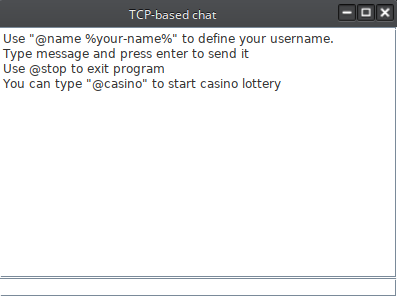
\includegraphics[scale=0.8]{chat1.png}}
		\caption{Окно клиента}
	\end{flushleft}
\end{figure}

\subsection{Пример общения клиентов}
\begin{figure}[H]
	\begin{flushleft}
		\centerline{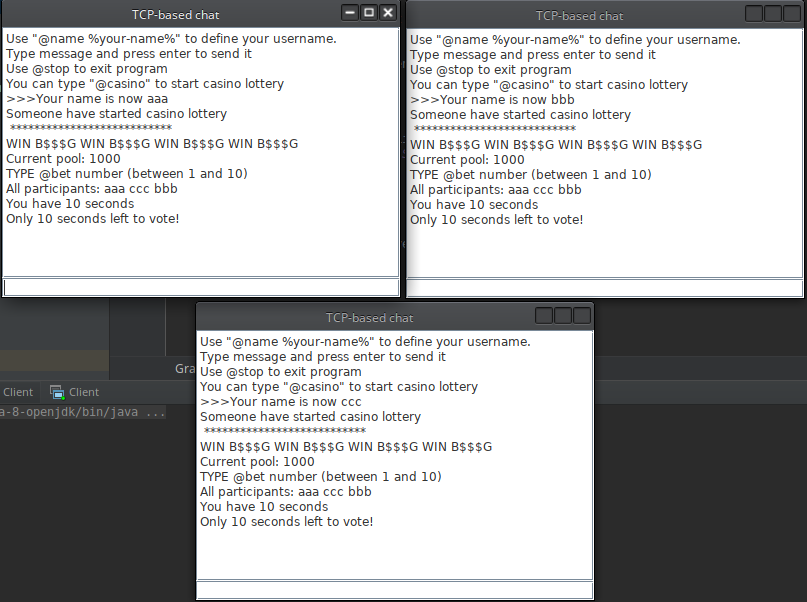
\includegraphics[scale=0.6]{chat2.png}}
		\caption{Запуск розыгрыша казино}
	\end{flushleft}
\end{figure}

\end{document}
